\documentclass[11pt]{scrartcl}

\usepackage[sexy]{evan}
\usepackage{pgfplots}
\pgfplotsset{compat=1.15}
\usepackage{mathrsfs}
\usetikzlibrary{arrows}
\usepackage{graphics}
\usepackage{tikz}
\usepackage{ amssymb }
\usepackage[dvipsnames]{xcolor}
\usepackage[utf8]{inputenc}
\usepackage{longtable}
\usepackage{ragged2e}
\usepackage{listings}


\definecolor{noseve}{RGB}{242,242,242}

\newcommand{\camod}[1]{\frac{\ZZ}{#1 \ZZ}}
\newcommand{\modm}[1]{\text{ mod } #1}
\newcommand{\campm}[1]{\frac{\ZZ}{m\ZZ}}

\usepackage{epigraph}
\renewcommand{\epigraphsize}{\scriptsize}
\renewcommand{\epigraphwidth}{60ex}


\definecolor{dcol0}{HTML}{C8E6C9}
\definecolor{dcol1}{HTML}{D4E9B3}
\definecolor{dcol2}{HTML}{E5ED9A}
\definecolor{dcol3}{HTML}{FFF59D}
\definecolor{dcol4}{HTML}{FFE082}
\definecolor{dcol5}{HTML}{FFCC80}
\definecolor{dcol6}{HTML}{FFAB91}
\definecolor{dcol7}{HTML}{F49890}
\definecolor{dcol8}{HTML}{E57373}
\definecolor{dcol9}{HTML}{D32F2F}

\makeatletter
\newcommand{\getcolorname}[1]{dcol#1}
\makeatother

\newcommand{\dif}[1]{%
    \edef\colorindex{\number\fpeval{floor(#1)}}%
    \edef\fulltext{#1}%
    \colorbox{\getcolorname{\colorindex}}{%
        \ifnum\colorindex>8
            \textbf{\textcolor{white}{\,\fulltext\,}}%
        \else
            \textbf{\textcolor{black}{\,\fulltext\,}}%
        \fi
    }%
}
% Variable para dificultad (inicial 0)
\newcommand{\thmdifficulty}{0}

% Comando para asignar dificultad antes del problema
\newcommand{\problemdiff}[1]{\renewcommand{\thmdifficulty}{#1}}

% Estilo del problema que incluye dificultad antes del título
\declaretheoremstyle[
    headfont=\color{blue!40!black}\normalfont\bfseries,
    headformat={%
      \dif{\thmdifficulty}\quad \NAME~\NUMBER\ifx\relax\EMPTY\relax\else\ \NOTE\fi
    },
    postheadspace=1em,
    spaceabove=8pt,
    spacebelow=8pt,
    bodyfont=\normalfont
]{problemstyle}

    \declaretheorem[style=problemstyle,name=Problema,sibling=theorem]{problema}
    \declaretheorem[style=problemstyle,name=Problema,numbered=no]{problema*}

%\usepackage[
%backend=biber,
%style=alphabetic,
%sorting=ynt
%]{biblatex}
%\addbibresource{referencias.bib}

\newcommand{\indicacion}[1]{\noindent\textit{\small #1}}


\title {Practica 6: Practica de arduino y shield Ethernet}
\subtitle{Unidad II: Interfaces de comunicación Tema 2.1 \\ Sistemas Embebidos II 18MPEDS0729 \\ Ago-Dic 2025 \\ Centro de Enseñanza Tecnica Industrial Plantel Colomos\\Tgo. en Desarrollo de Software \\ Academia: Sistemas Digitales \\Profesor: Antonio Lozano Gonzáles }
\date{19 de Octubre de 2025}
\author{Emmanuel Buenrostro 22300891 7F1 \\ \and Emiliano Arzate 22300929 7F1 \\}


\begin{document}

\maketitle
\begin{center}
   
\includegraphics[scale=0.15]{../../cetilogo.jpg} 
\end{center}
\newpage

\section{Objetivo}
Controlar relevadores por medio de internet, para manipular cualquier  tipo de carga y encender y/o apagar aparatos a distancia.
\section{Desarrollo de la Práctica}

\subsection{Condiciones de la Práctica}
Consiste en usar dos relevadores, los cuales serán controlados desde una pagina web. Se deberá utilizar un Arduino y
una shield ethernet. Por lo tanto se deberá tener  en dicha pagina mínimo dos botones, uno dirá relevador 1 ON/OFF; el otro botón dirá relevador 2 ON/OFF. Se pueden utilizar más botones si así lo desean. O en vez de botones perillas etc. usen su imaginación.
Un relevador sera para controlar un foco incandescente y el otro relevador controlara un ventilador

\subsection{Algoritmo o Diagrama de Flujo}

\begin{itemize}
  \item Inicializa comunicación serie, pines de relés como salida y los pone en estado HIGH (apagados).
  \item Configura la interfaz Ethernet con dirección MAC e IP y arranca un servidor en el puerto 80.
  \item En el bucle principal espera clientes entrantes del servidor.
  \item Cuando llega un cliente, lee la petición HTTP carácter por carácter y la acumula en una cadena.
  \item Si detecta rutas con parámetros (?rele1=on/off, ?rele2=on/off) actualiza los pines correspondientes y variables de estado.
  \item Cuando termina de leer la cabecera HTTP responde con una página HTML que muestra botones para encender/apagar según el estado actual.
  \item Cierra la conexión con el cliente y vuelve a esperar nuevos clientes.
\end{itemize}

\subsection{ Código C}

\lstinputlisting[language=C]{Pr6.ino}


\section{Observaciones y Conclusiones}

\begin{itemize}
    \item Usamos por primera vez el arduino como local para poder generar una pagina web. 
    \item Esto le dio una IP al arduino. 
\end{itemize}
  

\section{Imagen}

\begin{center}
    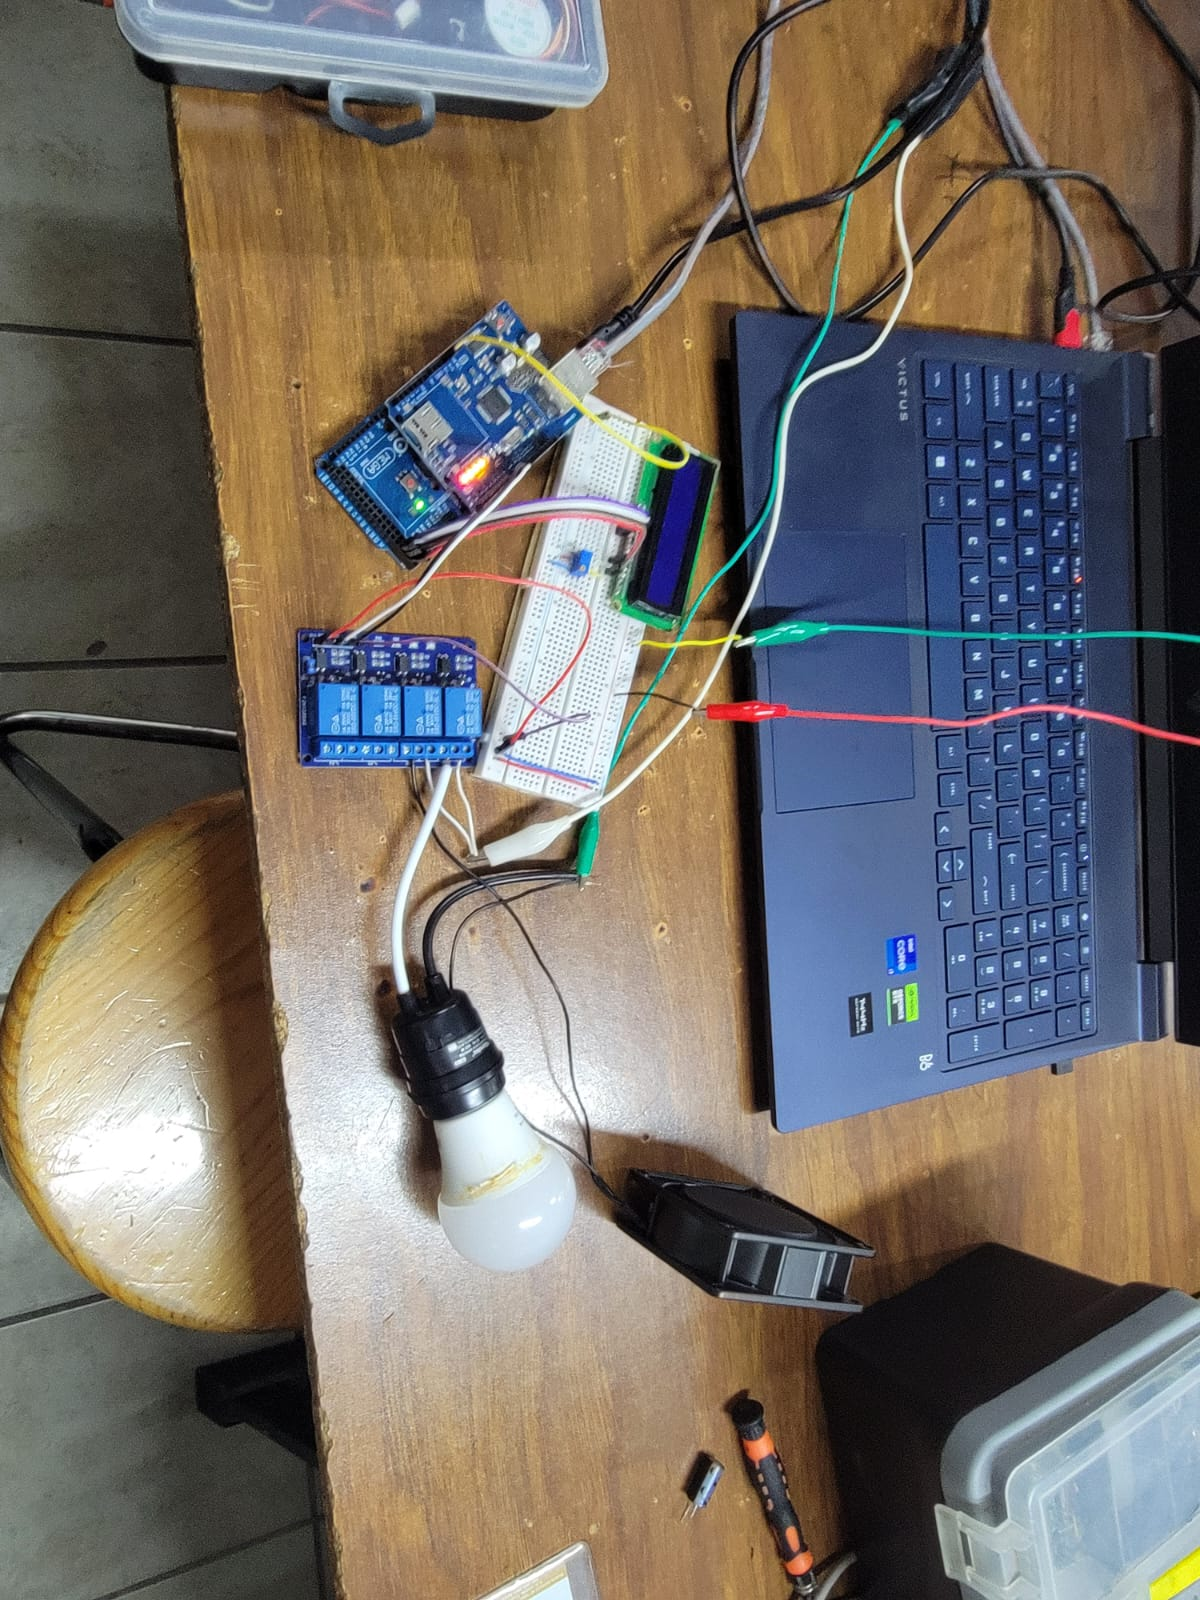
\includegraphics[scale=0.3]{imagen_circuito.jpg}
\end{center}
%\nocite{*}

%\printbibliography[
%heading=bibintoc,
%title={ . }
%]
    \end{document}